\Chapter{Megvalósítás}

\Section{Processz adatok lerkérdezése kernel modullal}

Az optimalizáláshoz szükség van adatokra a processzekről, amelyeket egy kernel modul segítségével könnyedén kinyerhetünk.
Mint ahogy \aref{ch:scheduling}. fejezetben láthattuk, minden processzhez tartozik egy vruntime változó, ami alapján történik a processzek megválasztása. 
Kernel modul segítségével a processzek tulajdonságai, mint például a \texttt{vruntime}, prioritás, súly és egyéb információk egyszerűen lekérdezhetők.
A kernelben processzek egy duplán láncolt listában tárolódnak, amit úgy hívnak hogy \textit{Processz tábla}. Minden egyes elem a listában egy \texttt{task\_struct} típusú processz descriptor, amit a \texttt{<linux/sched.h>}-ban defináltak. Egy processzről minden információ elérhető ezen keresztül.

\begin{figure}[h!]
\centering
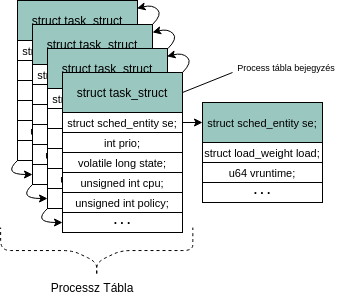
\includegraphics[scale=0.75]{images/processTable.png}
\caption{Processz Tábla}
\label{fig:structurehierarchi}
\end{figure}

\noindent A processz táblán a \texttt{for\_each\_process} makróval, egyszerűen végighaladtunk.
\begin{cpp}
struct task_struct *p;
#define for_each_process(p) \
	 for ( p = &init_task ; ( p = next_task(p)) != &init_task ; )
\end{cpp}
A \texttt{printk()}-függvényt használtam, a processz adatok naplózására.
\begin{cpp}
for_each_process(p)
    if(!p->rt_priority)
        printk(KERN_INFO
        "command: %s, pid:%d, priority: %d, weight: %lu, vruntime: %llu",
        p->comm, p->pid, p->prio, p->se.load.weight, p->se.vruntime);

\end{cpp}

Amennyiben az ütemező módosításokat közvetlenül a kernelben szeretnénk elvégezni, a változtatások után újra kell fordítanunk a kernelt.
Ez sajnos elég hosszadalmas lehet, emiatt másik megoldást választottam.

\Section{Processzor magok elszigetelése}

Szeretnék megemlíteni egy másik optimalizálási lehetőséget, mielőtt a kernel változók módosításába kezdünk. Úgy gondolom, hogy egyszerűen elvégezhető és szép teljesítmény növekedés nyerhető a következő módszerrel.
%TODO referencia: https://hu.wikipedia.org/wiki/Red_Hat_Enterprise_Linux
A Red Hat egy nyílt forráskódú szoftverek fejlesztésével foglalkozó vállalat. A Red Hat Enterprise Linux (rövidítve RHEL), a Red Hat által készített, kereskedelmi felhasználásra szánt Linux-disztribúció.
%TODO referencia https://access.redhat.com/documentation/en-US/Red_Hat_Enterprise_Linux/7/pdf/Performance_Tuning_Guide/Red_Hat_Enterprise_Linux-7-Performance_Tuning_Guide-en-US.pdf
A Red Hat által kiadott RHEL7 teljesítményre való hangolás útmutatójában, olvashatunk egy olyan módszerről, amellyel elkülöníthetünk processzorokat a ütemezőtől. Ezáltal elérhetjük azt, hogy az elkülönített processzorokon csak az általunk kiválasztott processzek futhatnak. Megvalósíthatjuk azt is, hogy egy processzhez több CPU magot rendelünk, így az izolált processzorokon nem lesz sok vetélytársa, akivel versengenie kellene az erőforrásért, emiatt teljesítménynövekvést tapasztalhatunk.
Ezt főként több CPU maggal rendelkező számítógépek esetén érdemes alkalmazni.

Egy processzor mag izolálást többféleképpen is megvalósíthatunk egy GNU/Linux operációs rendszerben.
Legegyszerűbben úgy érthetjük el, hogyha a bootolási paramétereket módosítjuk. Például a harmadik és a hatodiktól, a nyolcadik processzor mag izolálásához elegendő csak \texttt{/etc/default/grub} fájlt módosítanunk a következő képpen.

\begin{python}
GRUB_CMDLINE_LINUX_DEFAULT="isolcpus=2,5-7"
\end{python}

CPU izolációhoz használhatjuk még a tuna programot, amivel bármikor végrehajthatjuk ezt a műveletet és nem csak bootoláskor érvényesülnek a változtatások. Azonban ez a módszer kicsit máshogy működik mint az isolcpus paraméter, amit láthattunk az előbb. Egy CPU mag izoláció futás alatt azt eredményezi, hogy az aktuális CPU-hoz rendelt processzek, átkerülnek egy másikra és ezután végzi el az elszigetelést.

Az elszigelt processzorokhoz a taskset program segítségével tudunk manuálisan hozzárendelni processzeket. Amennyiben egy PTS programmal szeretnénk elindítani a stream benchmarkot, a harmadik processzor magon, azt a következő képpen tehetjük meg.

\begin{python}
$ taskset -c 2 phoronix-test-suite benchmark stream
\end{python}%$

A taskset programmal izoláció nélküli processzorokhoz is rendelhetünk processzeket, viszont így nem biztos, hogy annyira jelentős lesz a teljesítmény javulás.
A RedHat útmutatóban olvashatunk egy \texttt{numactl} programról amivel szintén hasonló eredményt érhetünk el, mint a \texttt{taskset} programmal. Itt viszont van egy probléma, mivel amennyiben elszigetelt processzorhoz szeretnénk rendelni processzt, hibát kapunk.
A \texttt{numactl} program ugyanis más logikát követ, amit láthatunk a következő kódrészletből.

\begin{cpp}
static struct bitmask *
__numa_parse_cpustring(const char *s, struct bitmask *allowed_cpus_ptr)
{
	int invert = 0, relative=0;
	int conf_cpus = numa_num_configured_cpus();
	char *end;
	struct bitmask *mask;

	mask = numa_allocate_cpumask();

	if (s[0] == 0)
		return mask;
	if (*s == '!') {
		invert = 1;
		s++;
	}
	if (*s == '+') {
		relative++;
		s++;
	}
	do {
		unsigned long arg;
		int i;

		if (!strcmp(s,"all")) {
			copy_bitmask_to_bitmask(allowed_cpus_ptr, mask);
			s+=4;
			break;
		}
		arg = get_nr(s, &end, allowed_cpus_ptr, relative);
		if (end == s) {
			numa_warn(W_cpuparse,
			 "unparseable cpu description `%s'\n", s);
			goto err;
		}
		if (!numa_bitmask_isbitset(allowed_cpus_ptr, arg)) {
			numa_warn(W_cpuparse, 
			"cpu argument %s is out of range\n", s);
			goto err;
		}
		...
\end{cpp}

Először kiolvassa a CPU affinitás-maszkot, és ezzel ellenörzi, hogy a megadott CPU-lista érvényes-e és csak akkor végzi el a processz CPU-hoz való rendelését, amikor ez érvényes.
Ezzel szemben a \texttt{taskset} programnak kicsit egyszerűbb a logikája.

\begin{cpp}
static void do_taskset(struct taskset *ts, size_t setsize, 
						cpu_set_t *set){
	/* read the current mask */
	if (ts->pid) {
		if (sched_getaffinity(ts->pid, ts->setsize, ts->set) < 0)
			err_affinity(ts->pid, 1);
		print_affinity(ts, FALSE);
	}

	if (ts->get_only)
		return;

	/* set new mask */
	if (sched_setaffinity(ts->pid, setsize, set) < 0)
		err_affinity(ts->pid, 1);

	/* re-read the current mask */
	if (ts->pid) {
		if (sched_getaffinity(ts->pid, ts->setsize, ts->set) < 0)
			err_affinity(ts->pid, 0);
		print_affinity(ts, TRUE);
	}
}
\end{cpp}

Először beolvassa az affinitás értéket, majd közvetlenül megvalósítja a processz affinitását, a \texttt{sched\_setaffinity} rendszerhívással.
A sikeres processzor elszigetelést ellenörizhetjük a \texttt{htop} programmal, amint egy nagyobb terhelést valósítottunk meg a számítógépünkön.

\begin{figure}[h!]
\centering
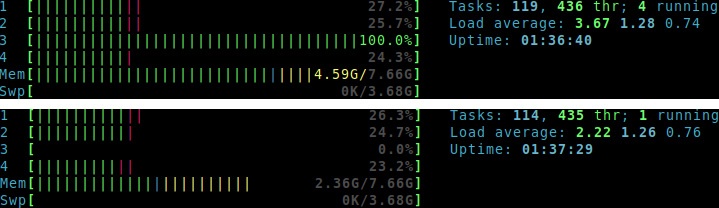
\includegraphics[width=\textwidth]{images/tasksetHtop.png}
\caption{Processz hozzárendelése egy izolált processzorhoz}
\label{fig:taskset}
\end{figure}

A másik módszer egy kicsit egyszerűbb, az elszigetelt CPU magokat megtalálhatjük a \texttt{/sys/devices/system/cpu/isolated} fájlban, vagy arra is van lehetőségünk, hogy az ellentétét listázzuk ami a \texttt{/sys/devices/system/cpu/present} fájlban található.

\Section{Ütemező módosítása}
Az alapvető cél a Linux processz ütemező optimalizálása, különféle használati módokra.
Ennek eléréséhez megtehetem, hogy módosításokat végzek az ütemezőn, amit elvégezhetek úgy hogy, konkrétan a forráskódot írom át, ezután újra lefordítom a kernelt és megfigyelem a módosítások hatásait.
A probléma, hogy a fejlesztési folyamat így nehézkes lehet, emiatt kerestem más módszereket.
Megfigyeltem, hogy több változó is elérhető az ütemező hangolására, így nincs szükség arra, hogy újakat vezessek be.

Ezeket a változókat megtalálhatjuk a \texttt{/proc/sys/kernel/} jegyzékben. Fontos kiemelni, hogy ezek a változók futásidőben is módosíthatók. Minden változóhoz tartozik egy intervallum, amin belül tetszőlegesen módosítható az értéke. 

Az értékek módosítását megadhatjuk direkt:
\begin{python}
$ echo $value > /proc/sys/kernel/sched_min_granularity_ns
\end{python}%$

A másik lehetőség, a \textit{sysctl} interfészen keresztül történő megadás:
\begin{python}
$ sudo sysctl -w sched_latency_ns=VALUE
\end{python}%$
A \textit{sysctl} interfész segítségével lekérdezhetem, módosíthatom a kernel változók aktuális értékeikeit és figyelmeztet arra is, hogy az adott változó értékét ne állítsam az intervallum végpontjain túllépő értékekre.
Az ütemező használati módokra történő optimalizálási kísérletemben, a \textit{sysctl} interfészen keresztül elérhető változók játszanak fő szerepet. Az ütemezőhöz tartozó változók, amik a \textit{sysctl} segítségével elérhetők a következők.

%https://elixir.bootlin.com/linux/v5.8.5/source/Documentation/scheduler/sched-design-CFS.rst
\begin{itemize}
\item \texttt{sched\_latency\_ns}

Ez a paraméter akkor játszik nagy szerepet, hogyha a processzek darabszáma a runqueue-ban, kisebb mint az \texttt{nr\_latency}. Fontos, hogy ez az érték nem összetévesztendő az időszelet méretével mivel, annak a számítását már láthattuk a \aref{sec:cfs}. szakaszban. 

\item \texttt{sched\_min\_granularity\_ns}

Ez a változó gyakorlatilag nagy processz szám esetén próbál meg egy minimális időszeletet biztosítani a processzek számára. Emiatt feltételezhetjük azt is, hogy végtelen processz szám esetén is, legalább egy milliszekundumot futással tölthet minden folyamat.

\item \texttt{sched\_wakeup\_granularity\_ns}

Ez az a minimális idő amelynek el kell telnie, mielőtt a CFS ütemező fontolóra veszi, hogy egy nagyobb \texttt{vruntime} értékkel rendelkező futtatható állapotú folyamattal leváltja, a jelenleg végrehajtás alatt álló taszkot.
Ez az opció késlelteti a preempció hatásait és csökkenti a túlütemezést. 

\item \texttt{sched\_tunable\_scaling}

Az ütemező hangoló paramétereket milyen mértékben befolyásolhatja, ehhez három féle opció is rendelkezésre áll.
\begin{enumerate}
\item \texttt{SCHED\_TUNABLESCALING\_NONE}

Itt nem történik módosítás, marad az eggyel való szorzás.
\item \texttt{SCHED\_TUNABLESCALING\_LOG}

Logaritmikus módosítás $*1+ilog(ncpus)$
Ahol az \texttt{ncpus} a cpu-k számát jelöli.

\item \texttt{SCHED\_TUNABLESCALING\_LINEAR}

Lineáris módosítás, $*ncpus$. 
\end{enumerate}

\item \texttt{sched\_cfs\_bandwidth\_slice\_us}

A CFS bandwidth control szabályozza a futási idő mennyiségét, amelyet a taszk csoportjának sávszélesség-készletéből helyeznek át runqueue-ba. A kis értékek lehetővé teszik a globális sávszélesség aprólékos megosztását a folyamatok között, a nagyobb értékek csökkentik az átviteli költségeket.
%TODO refrencia: https://elixir.bootlin.com/linux/v5.8.5/source/kernel/sched/fair.c
\item \texttt{sched\_child\_runs\_first}

Egy fork rendszerhívás után, a gyerek processz kezd el futni először ha, ennek a paraméternek az értéke egyre van állítva. Nulla esetén (ami az alapértelmezett beállítás) a szülő processz próbál meg először futni, de előfordulhat, hogy nem sikerül neki.

\item \texttt{sched\_migration\_cost\_ns}

Az utolsó végrehajtás után eltelt idő, ameddig a feladatot „gyorsítótár-frissnek” tekintik.
Egy ilyen friss taszk-nál kevésbé valószínű, hogy az ütemező átvinné egy másik CPU-ra, szóval a változó értékének növelése, csökkenti ezt az esélyt.
\item \texttt{sched\_nr\_migrate}

Az a maximális taszk szám, amit a kiegyensúlyozási eljárás során kezel az ütemező.
\item \texttt{sched\_rr\_timeslice\_ms}

Az időszelet mérete, amit futással tölthet mielőtt preemptálja az ütemező és a taszk lista végére kerül.
\item \texttt{sched\_rt\_period\_us}

A CFS ütemező ennyi időt vár, mielőtt odaadná a CPU-t valamelyik valós idejű taszknak újra.
\item \texttt{sched\_rt\_runtime\_us}

Az a maximális processzor idő amit felhasználhat egy valós idejű taszk.
\end{itemize}
A felsorolt paraméterek közül a \texttt{sched\_latency\_ns}, \texttt{sched\_wakeup\_granularity\_ns} és a \texttt{sched\_wakeup\_granularity\_ns} kap nagyobb figyelmet a dolgozatban. Ezek mellett még a processzek prioritási szintjét fogom módosítani, amivel a vruntime számításnál találkozhatunk.
Az utolsó változó pedig a \texttt{vm.swappiness}, amit szintén elérhetünk a \textit{sysctl} interfész segítségével. 

A \texttt{vm.swappiness} egy hangolható kernelparaméter, amely szabályozza, hogy a kernel mennyire kedvez a swap memóriának a RAM felett. A változó intervalluma 0-100 ig terjed, magasabb érték agresszív kilapozást eredményez, amíg a nullánál pedig mondhatni teljesen ki lesz kapcsolva a swap memória használata. Az összes ütemezőhöz kapcsoló hangolható paraméter tesztelése túl sok időt vehet igénybe, feltéve azt, hogy minden beállítással szeretnék futtatni egy tesztet és egyes paraméterek intervallumai sem mondhatók túl kicsinek. Ezért a kiválasztott paramétereim intervallumát négy részre fogom szétszedni, annak érdekében, hogy a tesztek hamarabb lefussanak, így több időt tudok szánni a kapott adatok elemzésére.

A módosítások hatásait benchmark programokkal tervezem mérni, amelyhez a PTS programot fogom felhasználni. Mivel különböző felhasználási módokra tervezem az optimalizálást, így az \texttt{openbenchmarking.org} oldaláról minden kategóriából választottam egy tesztet. 
Teszt választásnál fő szempont volt a gyors lefutási idő, a teszt müködése és hogy milyen konfigurációs beállítások elérhetők hozzá. Annak érkében, hogy pontos mérést végezzek a tesztekkel, célszerűnek tartottam azt, hogy minden változó módosításnál több mintát is vegyek.
Mivel kézzel a tesztek indítása és a paraméterek megváltoztatása egyesével elég hosszadalmas lenne, így készítettem erre egy programot.

\Section{A \textit{Parameter-test} program}

A program, C programozási nyelven \texttt{ncurses} és \texttt{xml} library-k használatával készült.
A feladata, hogy módosítsa a kernel paramétereket, illetve a prioritást, az adott beállítással elindítson, adott darabszámot a tesztből és az eredményeket lementse, majd ezeket a lépéseket minden iterációban megismételje emberi beavatkozás nélkül.

Azért a C programozási nyelvet válaszotttam a megvalósítására, mert a processz prioritási tulajdonságok, illetve a \textit{sysctl} interfész is egyszerűen kezelhető vele.

\SubSection{A program felépítése}

A program először inicializálja az \texttt{ncurses} képernyőt, majd ezután meghívja az első fő függvényt, aminek a feladata, hogy bekérje a felhasználótól a teszt nevét verziószámmal együtt. Ezután a mintaszámot, illetve az intervallum szétbontásának számát kéri be.  

\begin{cpp}
void initTestVariables(char *testName, int *sampleCount, int *interval)
\end{cpp}

Az utóbbi két input átugorható enter megnyomásával, ekkor alapértelmezett öt mintát fog venni és öt részre fogja szétszedni az intervallumokat.

\begin{figure}[h!]
\centering
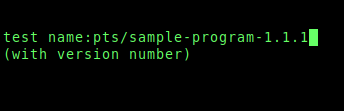
\includegraphics[scale=3.0]{images/parameter-testInit.png}
\caption{\textit{Parameter-test program}, tesztnév megadás}
\label{fig:parameter-testInit}
\end{figure}

A tesztnév megadásnál fontos a veriószám megadás, mivel a tesztekből újabb változatok kerülnek fel a \texttt{openbenchmark.org}-ra és minden verzióhoz új jegyzéket készít a PTS program a /var/lib/phoronix-test-suite/test-profiles/pts directory-ba.
Minden teszthez tartozik egy jegyzék, amiben több \texttt{xml} kiterjesztésű fájl is megtalálható, ezek közül fontos kiemelni a \texttt{test-definition.xml}-t amiben a teszthez tartozó konfigurációs beállítások találhatók meg.
A kezdeti paraméterek megadását követően, a teszt előkészületeihez ér a program, itt történik meg a teszt név ellenörzése, elérhető teszt konfigurációk listázása, kiválasztása és a \textit{batch-benchmark} benchmark indítási módszer konfigurálása. 

\begin{cpp}
void preparations(char *testName)
\end{cpp}

A \texttt{sched\_tunable\_scaling} kernel változó alapértelmezett értéke 1, amiről megtudhattuk az elöző pontban hogy, bizonyos mértékben módosítani fogja a beállított kernel változókat a teszt során, emiatt én \texttt{preparations} függvényem elején, ezt az értéket 0-ra állítom. Így biztosítom azt hogy véletlenül se legyen emiatt, benchmarkból származó inkonzisztens értékem.
Ezt követi a tesztnév-verziószám ellenörzés. Amennyiben nem találja meg a megadott névvel a fájlt, a program hibaüzenettel leáll.
Abban az esetben, ha létezik a fájl és a hozzá tartozó teszt, a konfigurációs beállításokat meg kell jelenítsem illetve módosítanom kell azokra az értékekere, amelyeket a felhasználó kiválaszt.
A PTS programban két féle képpen lehet beállításokat megadni úgy, hogy ne szakítsa meg a végrehajtást amiatt, hogy újra bekéri billentyűzetről a megadott opciót.
\begin{enumerate}
\item A PTS dokumentációban olvashatunk arról, hogy van lehetőségünk környezeti változónkon keresztül megadni. Több ilyen változó elérhető, azonban a teszt opciók beállítására a \texttt{PRESET\_OPTIONS}-t használjuk. A megadási mód egyszerűnek mondható, több paraméter esetén pontosvesszűvel elválaszthatjuk az opció beállításokat. A beállítást a következő képpen történik.
\begin{cpp}
PRESET\_OPTIONS="stream.run-type=Add"
\end{cpp}
\item A másik módszer, amit a \textit{parameter-test} programban implementáltam, a konkrét konfigurációkat tartalmazó fájlt nyitom meg, és állítok be egy alapértelmezett értéket minden egyes opcióhoz. Ez a fájl a \texttt{/var/lib/phoronix-test-suite/} \texttt{test-profiles/pts/}tesztnév-verziószám\texttt{/} jegyzékben található \\ \texttt{test-definition.xml}. Sajnos néhány esetben előfordul hogy egy teszthez a PTS program valós időben lekérdezi az \texttt{openbenchmarking.org}-ról az opciókat és csak a beállítás nevét találjuk meg. Ebben az esetben is rákérdez a parameter-test program az opció beállítására, de a lehetséges választásokat csak az \\ \texttt{openbenchmarking.org}-on tekinthetjük meg.
\end{enumerate}
A beállítás mindkét módszerrel müködik, azonban számos olyan benchmark program szerepel a PTS programban, amihez egyáltalán nem is tartozik beállítható konfiguráció. A program a fájl írása után elmenti a módosításokat és sikeres írás után, következik a batch-benchmark konfiguráció. 
Ez a fájl a \texttt{/etc/phoronix-test-suite.xml}, amelyben a \texttt{<BatchMode>} node-ban található értékeket szükséges megfelelően testre szabnunk. Amennyiben ez a lépés elmaradna, a PTS program megállítaná a benchmark programot, hogy bekérje az értékeket. Ezzel el is értünk a teszt indításához, ennél a pontnál a szükséges beállításokat már elvégezte a program.
\begin{cpp}
void startTest(int interval, int sampleCount, char *testName);
\end{cpp}
A főbb paraméterek átadása meghatározza a kimeneti fájl nevét, amibe belefűzi a dátumot (év, hónap, nap, óra, perc, másodperc), így több teszt is futtatható egymást követően, anélkül hogy felülírnák egymást.
Ezt követően a kernel változók inicializálásra kerülnek, mind a saját intervallumának a legkisebb értékét veszi fel. A program a ciklusmagban, készít egy menüt, amibe kiírja a teszt nevét, a teszt sorszámát és az utolsó öt eredményt, amit a teszt az aktuális beállításokkal produkált. A menü kirajzolása után elindul az első benchmark, a kívánt mintaszámmal és konfigurációs beállításokkal. Amikor a benchmark befejeződött, az eredményt eltárolja a \texttt{/var/lib/phoronix-test-suite/test-results/myresult/composite.xml} fájlban, \\ amelyből a program kiolvassa az eredményt, amit továbbít az eredmény fájlba, az aktuális kernel változókkal együtt. Ezt az eredményt továbbítja az eredmények oszlopba is, így a felhasználó is követheti az eredmények változását.

\noindent A program kiolvassa az eredményt, amit továbbít az eredmény fájlba, az aktuális kernel változókkal együtt. Ezt az eredményt megjeleníti az eredmények oszlopba, így a felhasználó is követheti az eredmények változását.

\begin{figure}[h!]
\centering
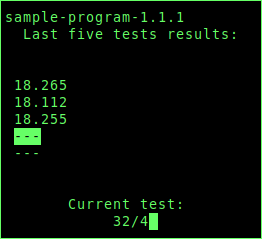
\includegraphics[scale=3.0]{images/parameter-test.png}
\caption{Parameter-test program utolsó eredmények}
\label{fig:parameter-test}
\end{figure}

Végül a menü ablakot törli és újrarajzolja a következő iterációban.
Amikor a teszt végzett az összes kernel változó végigpróbálásával, a fájlt lezárja és visszaállítja a változókat az eredeti értékükre.
Az így kapott fájl formátuma JSON típusú, amely előnyös a későbbi elemzés szempontjából.

\Section{\textit{SchedulerTuneML} program}
% \SubSection{\textit{SchedulerTuneML} program implentációja}

A \textit{SchedulerTuneML} program Python programozási nyelven készítettem, több különböző modul felhasználásával.
A program célja hogy, a \textit{parameter-test} program által készített JSON fájlokat feldolgozza. A fájlból kinyert adatokat elemzi, besorolja őket csoportokba, diagrammokat készít ezekből és javaslatokat tesz a kernel változók értékeinek beállítására, az adott felhasználási módhoz viszonyítva.

\SubSection{Adatok előkészítése az elemzéshez}

A program \textit{Jupyter} munkafüzetként készült, emiatt a fájlok \texttt{.ipynb} kiterjesztésüek. Kihasználva a notebook által készíthető cellákat, a legtöbb kódrészlet mellé készítettem leírásokat, úgy gondolom hogy egyszerűbben megérthetők ezekkel, az egyes kódrészletek.

A benchmark program által készített eredmények tesztenként eltérőek, ami főként a különböző felhasználási módból következik. Ezeket az értékeket normalizálnom kell először, mielőtt felhasználnám a model betanításánál. Ehhez \textit{feature scaling}-et alkalmaztam, ami azt jelenti hogy abban az esetben amikor a teszt értékek közül a kisebb érték számít jobbnak a következő képletet használom fel:
\begin{equation}
x = \frac{max-x}{max-min}.
\end{equation}
Amennyiben a nagyobb érték számít jobbnak, az előző képlett kicsit módosított változatát:
\begin{equation}
x = \frac{x-min}{max-min}.
\end{equation}
Ezek felhasználásával biztosítom, hogy az értékek nulla és egy között maradjanak, és a nagyobb értékek jelentsék az előnyös esetet.
A meglévő adathalmazom azonban önmagában nem elegendő arra, hogy a neurális hálót be tudjam tanítani vele, emiatt új elemeket, illetve kategóriákat vezettem be.
\begin{itemize}
\item \textit{resultClass}

A program első lépései, a JSON fájlok megnyitása, az értékeken történő végigiterálás, annak érdekében, hogy megtaláljam a legkisebbet, illetve a legnagyobbat. Ezt követően létrehozok 5 szintet az értékek csoportosítására, amely a következő képpen történik.
\begin{alignat*}{2}
         x& < 20 &: 0 \\
    20 < x& < 40 &: 1 \\
    40 < x& < 60 &: 2 \\
    60 < x& < 80 &: 3 \\
    80 < x& < 100&: 4
\end{alignat*}
A legrosszabb értékek kategóriája gyakorlatilag $floor(x / 20)$ formában is számítható.

\item \textit{serverWorkload}

A Linux kernel dokumentációjában olvashatunk az ütemezőt behangolhatjuk, szerver szintű terhelésre. Ezt az eredményt, a \texttt{sched\_min\_granularity\_ns} kernel változó módosításával érhetjük el.
Mivel a szerver szintű terheléseknél, sűrűbben fordulnak elő batch processzek, azaz akik életük nagyrészét inkább számításokkal töltik és náluk előnyösebb nagyobb időszeleteket használni. Ezt az eredményt pedig elérhetjük ennek a változó módosításával. Így amikor nagyobb értéket vesz fel a \texttt{sched\_min\_granularity\_ns} mint az alapbeállítás, serverWorkload kategóriába kerül.
\item \textit{swap} 

A \texttt{swap} csoport gyakorlatilag a swap memória igényt jelzi. 
Minden olyan mérési eredményt, amelynél nem fordult elő swap memória használat, nullával láttam el, ellenkező esetben pedig egyessel.
\item \textit{batchProcess}

Batch processzek, nem szükséges nagy prioritást állítani, kevesebbszer kerülnek végrehajtásra, viszont ekkor nagyobb időszeletet is kaphatnak. Emiatt hogyha egy processz prioritása nagyobb mint nulla, \textit{batchProcess} kategóriába kerül.
\end{itemize}

A felsorolt kategóriák, fontos részét képezik az adathalmaznak amit kialakítottam. Ebbe az adathalmazba szintén beletartoznak a benchmarkokból származó eredmények, amik átestek a feature scaling-en, illetve a hozzá tartozó kernel változók. Az adathalmazból egy \texttt{DataFrame}-et készítettem, a \textit{Pandas} modul segítségével. Ezáltal egyszerűen átláthatom, lekérdezhezhetek belőle részeket, és ábrázolhatom az adatokat.
Az így kapott \texttt{DataFrame} segítségével fogom megkísérelni egy neurális hálózat betanítását. 
%TODO referencia könyvből: Hands-On Machine Learning with Scikit-Learn, Keras, and TensorFlow: Concepts, Tools, and Techniques to Build Intelligent Systems 2nd Edition
\SubSection{A gépi tanulás megvalósítása}
A gépi tanulásra egy lehetséges definíció a következő.

\begin{quote}
``A gépi tanulás az a tanulmányi terület, amely képessé teszi a számítógépeket a tanulásra
anélkül, hogy kifejezetten beprogramozták volna.''
\par\nobreak\smallskip\hfill—Arthur Samuel, 1959
\end{quote}

A gépi tanulásnál számos területe létezik. Az aktuális probléma megoldására felügyelt tanítást alkalmaztam. Ez azt jelenti, hogy az adathalmazban az egyes mintáknál, megtalálhatók a jellegek (\textit{features}), illetve az elvárt eredmények is (\textit{labels}).

Mivel a kernel változók intervallumait négy részre szedtem szét a teszteléseknél, így erre egy klasszifikációs algoritmust használok fel.
A modelt az adott problémához mérten kell felépíteni, amihez fontos, hogy optimálisan válasszuk meg rejtett rétegek, illetve a neuronok számát.
Esetemben, a model öt bemenettel, illetve öt kimenettel rendelkezik, és egy rejtett réteget választottam a topológia kialakításához (\ref{fig:neuralnetwork}. ábra).

\begin{figure}[h!]
\centering
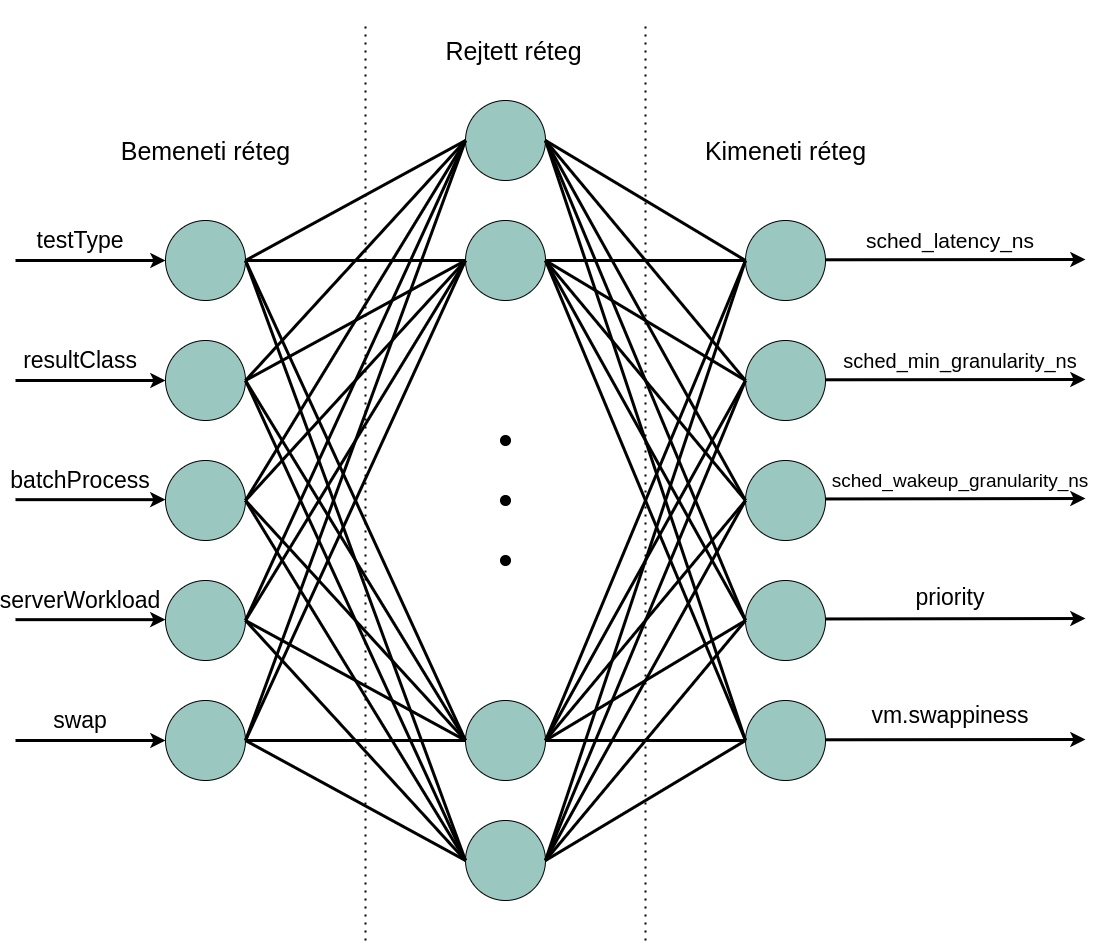
\includegraphics[width=\textwidth]{images/neuralNetwork.png}
\caption{Neurális hálózat}
\label{fig:neuralnetwork}
\end{figure}

Alapvetően ezek a mesterséges neuronok, fogalmilag biológiai idegsejtekből származnak.
Minden neuron több bemenettel rendelkezik és egyetlen kimenettel, amit több neuronnak is képes továbbítani.

\noindent A neuron által kiszámított kimeneti érték \aref{fig:neuron}. ábrán látható módon határozható meg.
\begin{figure}[h!]
\centering
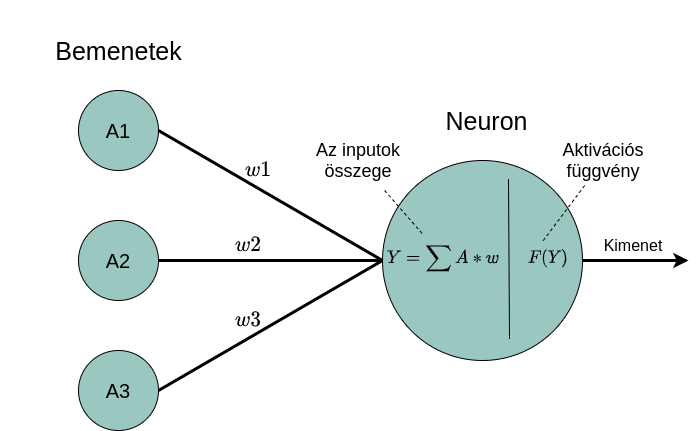
\includegraphics[scale=0.5]{images/neuron.png}
\caption{Neuron}
\label{fig:neuron}
\end{figure}

Az inputokat beszorozzuk a hozzájuk tartozó súlyokkal, majd ezeket összeadjuk és az így kapott értéket behelyettesítjük az aktivációs függvénybe.
%TODO referencia: https://towardsdatascience.com/activation-functions-neural-networks-1cbd9f8d91d6
Az aktivációs függvénnyel elérhetjük hogy az érték 0 és 1 között maradjon, vagy néhány esetben -1 és 1 között (függvénytől függ). Ezzel határozzuk meg a neurális hálózat kimenetét, olyan mint hogyha azt mondanánk hogy igen vagy nem (vagyis történik aktiváció vagy sem). 
A következő aktivációs függvények közül választhatunk, az \textit{sklearn} osztályozó algoritmusához.
\begin{itemize}
\item \texttt{identity}, $f(x) = x$

Egy egyszerű lineáris függvény, értékkészlete $\mathbb{R}$.
\item \texttt{logistic} - $f(x) = \frac{1}{1+e^{-x}}$

Logisztikus vagy Szigmoid függvény, ami eg S alakot ír le. Az oka amiért előszeretettel használjuk ezt a függvényt az, hogy az értékkészlete pont 0 és 1 között található. Ez különösen azoknál a modelleknél alkalmazzák, ahol a valószínűséget kimenetként kell megjósolnunk.
\item \texttt{tanh} - $f(x) = \frac{e^{x}-e^{-x}}{e^{x}+e^{-x}}$

A tangens hiperbólikusz függvény nagyon hasonló a szigmoidhoz, de jobb nála. Az értékkészlete -1-től 1-ig tart, és ő is S alakú függvény.
A negatív részének nagy előnye van, mivel ezt vehetjük úgymond erősen negatívnak, azaz egy erős "nem" kimenetnek. Jellemzően klasszifikációs modelleknél használják ezt a függvényt.
\item \texttt{relu} (Rectified Linear Unit) - $f(x) = max(0,x)$

%A ReLU jelenleg a világon a leggyakrabban használt aktivációs függvény.
Az $f(x)$ függvény értéke nullát vesz fel, minden olyan esetben amikor $x$ értéke nulla vagy kisebb mint nulla és $f(x)$ értéke megegyezik $x$ értékével, ha $x$ nagyobb mint nulla.
A függvény értékkészlete $[0,\infty)$.
\end{itemize}

Amennyiben az adott modelben több rejtett réteg is található, az előző aktivációs függvény érték veszi fel a bemeneti érték szerepét és így halad tovább az algoritmus. Amikor sikeresen elértünk az kimeneti réteghez, a kapott eredményt összehasonlítjuk az elvárttal, ebből egy hibát számítunk.
Ekkor visszafele haladunk a modelben és a kapott hibával újraszámítjuk a súlyokat.
Ezután pedig ismételten előre iterálunk, az új súly értékeket felhasználva a neuron számításoknál.

A rejtett rétegben elhelyezkedő neuronok számának meghatározásához nincs semmiféle varázsképlet, azonban találtam néhány ökölszabályt, amik a következők. 
%TODO referencia könyvből: Introduction to Neural Networks with Java: page 129
\begin{itemize}
\item A rejtett rétegben lévő neuronok száma, a bemeneti és kimeneti rétegek méretei között kell, hogy essenek.
\item A rejtett rétegben lévő neuronok száma, legyen a bemeneti réteg méretének kétharmada, amihez hozzáadjuk a kimeneti réteg méretét.
\item A rejtett rétegben lévő neuronok száma, legyen kevesebb, mint a bemeneti réteg méretének a kétszerese.
\end{itemize}

%TODO referencia az sklearn oldaláról: https://scikit-learn.org/stable/modules/generated/sklearn.neural_network.MLPClassifier.html
Gépi tanulás algoritmusai gyakran támaszkodnak valamilyen célfüggvény optimalizálásra, ezért az optimalizálási algoritmus megválasztása a tanulás folyamat egyik fontos része.
Az \texttt{sklearn.neural\_network.MLPClassifier} esetén, három választásunk van.
\begin{itemize}
\item \textit{ADAM}, ami egy sztochasztikus gradiens alapú optimalizáló algoritmusra utal, amelyet még Kingma, Diederik és Jimmy Ba javasolt.
\item \textit{sgd} (stochastic gradient descent), amely a negatív gradiens irányába tesz lépéseket a célfüggvényhez.
\item \textit{L-BFGS}, egy  optimalizáló algoritmus a kvázi Newton-módszerek családjából
\end{itemize}

A rejtett réteghez tartozó neuron számot, aktivációs függvényt és optimalizálási algoritmust, az adott problémához mérten érdemes megválasztani. A legjobb paraméterek meghatározására készítettem egy halmazt, amibe elhelyeztem az összes aktivációs függvényt, optimalizálási algoritmust és néhány neuron számot, amelyek megfelelők lehetnek a feladat megoldásához.

\begin{python}
params = {
            'estimator__activation' : ['identity', 'logistic',
            			       'tanh', 'relu'],
            'estimator__solver' : ['lbfgs', 'sgd', 'adam'],
            'estimator__hidden_layer_sizes': [(1, ),(2, ),(3, ),
            				      (4, ),(5, ),(6, ),
            				      (7, ),(8, ),(9, ),
            				      (10,),(11,),(12,),
            				      (13,),(14,),(15,),
            				      (16,),(17,),(18,),
            				      (19,),(20,),(21,)]
}
\end{python}

\SubSection{Optimális paraméterek keresése}
A paraméterezés kapcsán az \texttt{sklearn.grid\_search.GridSearchCV} függvényt választottam, ami egy kimerítő keresést végez, a legjobb paraméterek megtalálásához. A függvény alkalmazásához készítenem kellett egy paraméter készletet, amiben végig próbálja az összes lehetséges kombinációját. Ami azt jelenti hogy, minden próba végén kiértékeli a modelt egy Cross-Validation módszer segítségével. Ezáltal megkaptam azokat a model paramétereket, amivel a legjobban teljesített.
%referencia az sklearn GridSearch és Cross Validation-re: https://scikit-learn.org/stable/modules/cross_validation.html
\begin{figure}[h!]
\centering
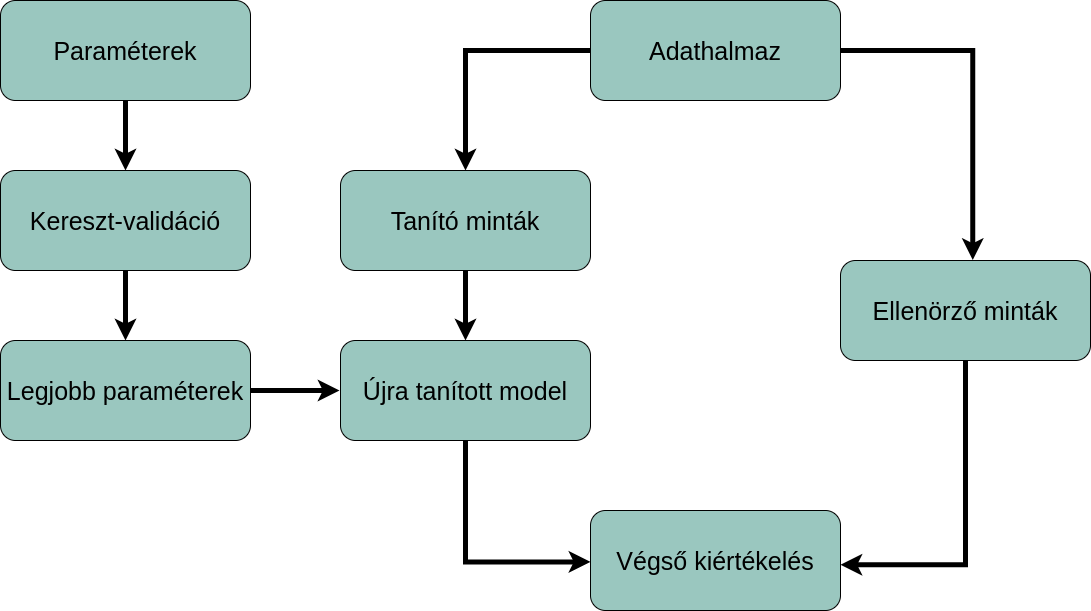
\includegraphics[scale=0.3]{images/gridSearch.png}
\caption{Kereszt-validáció, a paraméterek megkeresésére}
\label{fig:neuralnetwork}
\end{figure}

Minden próba végén kiértékeli a modelt egy Cross-Validation módszer segítségével. A legjobb értéket elért paraméterek, ezután lekérdezhetők a következő képpen.

\begin{python}
model = GridSearchCV( MultiOutputClassifier(MLPClassifier())
  ,param_grid=params)
model.fit(X_train,y_train)
print(model.best_params_)
\end{python} 

Az itt látható program kimenete alapján, választottam meg a paramétereket.
Így a tangens hiperbólikusz függvényt, használtam fel aktivációs függvényként, emellett kilenc neuront és az L-BFGS optimalizáló algoritmust alkalmaztam.

%TODO referencia könyvből: Hands-On Machine Learning with Scikit-Learn and TensorFlow
Az egyetlen módja, hogy kiderítsem hogyan teljesít a modell, ki kell hogy próbáljam új adatokkal. 
Ezt megtehetem úgy hogy késznek nyilvánítom a programot tanítás után és a felhasználók amikor majd kipróbálják, kiderül hogy sikerült. Ez az ötlet ugyan müködhet, de amennyiben a model rosszul lett felépítve meglehet hogy nagyon rosszul teljesít és a felhasználóknak nem fogja elnyerni a tetszésüket. Egy okosabb módszer a rendelkezésre álló adathalmazt, szétszedni két részre. Az első halmazban találhatók a tanító minták, amikkel a modell betanítását fogom végezni. A második halmaz ellenörzésre szolgál, ahol a mintákkal csak tesztelem a modell teljesítményét.
Ezeket \textit{training} és \textit{testing set}-nek is szokás nevezni, az utóbbi felhasználásával kiderülhet a hibaarány mérete, amit szokás általánosítási hibának is nevezni. Ez az érték megmondja, hogy a model mennyire fog jól teljesíteni olyan mintákon, amelyeket még nem látott korábban.
Amennyiben a model rosszul teljesített a tanító és az ellenörző mintákat tartalmazó adathalmazon egyaránt, fennállhat az alul tanulás problémája, erre egy megoldás lehet az hogyha komplexebb modelt tervezünk. Abban az esetben, ha jól teljesített a tanító mintákon, viszont rosszul az eddig még nem látottakon, előfordulhat hogy a model túl tanult. A cél a kettő között helyezkedik el, így erre nagy figyelmet kell model készítés során.
Gyakori, hogy az adatok 80\% -át használják fel tanításra, és a maradék 20\% -ot tesztelésre. Ez azonban az adatkészlet méretétől függ, amennyiben az adathalmazunk 10 millió példányt tartalmaz, elég lehet az adatok 1\% -át felhasználni tesztelésre, 100 000 példány valószínűleg több, mint
elég ahhoz, hogy jó becslést kapjunk az általánosítási hibáról. Az én esetemben az adathalmazomban 6144 minta található, emiatt én az adatok 80\%-át fogom felhasználni tanításra és a maradékot pedig a modell tesztelésére fordítom. Erre a célra az \texttt{sklearn.model\_selection.train\_test\_split} függvényt fogom felhasználni. 

\begin{python}
X = df[["testType","resultClass","batchProcess","serverWorkload","swap"]]
y = df[["latency","min_gran","wakeup_gran","priority","vm.swappiness"]]
X_train,X_test,y_train,y_test = train_test_split(X,y,test_size=0.2)
\end{python}

Paraméterként meg kell adjam a használati módokat (\texttt{X}), a hozzátartozó kernel változókat (\texttt{y}) és az tesztelési adathalmaz méretét \%-os formában.
Az \texttt{X} változó gyakorlatilag egy részlet a \texttt{DataFrame}-ből. %, ami látható a következő kódrészletből.

A \texttt{testType} az adott felhasználási módot jelöli, az elérhető felhasználási módok a benchmark kategória típusok. Az elérhető kategóriák a következők: 
\begin{enumerate}
\item Egy CPU magot igénylő, processzor igényes felhasználási mód.
\item Több CPU magot igénylő, magas processzor intenzitású felhasználási mód.
\item Rendszert terhelő felhasználási mód.(Sok rendszerhívásra lehet számítani)
\item Háttértárat terhelő felhasználási mód.
\item Memóriát és processzort terhelő felhasználási mód.
\item Videókártyát terhelő felhasználási mód.
\end{enumerate}

A \textit{resultClass} az eredmény besorolása, kategóriákba. Ezt az értéket mindig 4-re állítom, ezzel próbálom meg elérni hogy mindig a legjobb értékek közül kapjak paramétereket.

A \textit{batchProcess} paraméter segítségével beállítható hogy az adott processzt kívánja-e a felhasználó batch módban futtatni. Ez a processz prioritását és a processzhez tartozó vruntime változó értékének módosítását jelenti. A \textit{batchProcess} mód beállításhoz 1-re kell állítani a változó értékét, egyébként 0-ra.

A \textit{serverWorkload} segítségével a felhasználó a futtatni kívánt processzeihez mérten beszabályozhatja az ütemezőt. Amennyiben a processzek amiket futtatni szeretne, szerver szintű terhelési módhoz állnak közel, érdemes ezt a változót 1-re állítani, ellenkező esetben 0-ra.

A \textit{swap} paraméterrel, a felhasználó eldöntheti hogy szeretne-e swap memóriát használni. Érdemes lehet ezt a változót beállítani 1-re, kevés memóriával rendelkező számítógépek esetén. Abban az esetben ha nincs szüksége erre az opcióra, 0-ra kell beállítania az értéket.

A kimenet a paraméterkészlet az ütemező hangoláshoz, a futtatni kívánt processzekhez az ajánlott prioritás és swap memóriát szabályzó kernel paraméter, az adott felhasználási módhoz mérten.
A model létrehozása és betanítása a következőképpen történik az \textit{sklearn} függvénykönyvtár felhasználásával. 
\begin{python}
model = MultiOutputClassifier(MLPClassifier(
	solver="lbfgs",
	hidden_layer_sizes=(9,),
	activation="tanh"))
model.fit(X_train,y_train)
\end{python}
A hagyományos model létrehozása során elég csak az \texttt{MLPClassifier}-t meghívni, a kívánt paraméterekkel. Esetem viszont kicsit máshogy néz ki, a modellem több bemenettel, illetve kimenettel rendelkezik. A \texttt{MultiOutputClassifier} ezt valósítja meg, és paraméterként pedig egy \texttt{estimator}-t vár, ami jelen esetben nálam az \texttt{MLPClassifier}.

%TODO referencia a joblib-hez: https://scikit-learn.org/stable/modules/model_persistence.html
Annak érdekében, hogy a tesztelés gördülékenyebben menjen, a modelt előre betanítottam, így futtatáskor nincs szükség újra és újra elvégezni a tanítást.
A model lementéséhez, többféle lehetőség is rendelkezésre áll. Ehhez a \texttt{joblib} modult választottam, mivel sokkal hatékonyabb olyan objektumoknál, amik nagyobb méretű NumPy tömböket tartalmaznak és a \textit{sklearn} oldalán is ennek a használatát javasolják.
Két függvényt alkalmazok.
\begin{itemize}
	\item Az első a lementést valósítja meg \texttt{joblib.dump()}, ami paraméterként az elkészített modelt kapja meg és hogy milyen néven mentsük el.
\item A másik a betöltésért felel, itt egyszerűen csak a fájlnévre hivatkozunk.
\end{itemize}
Ahogy látható az alábbi kódrészletből, szintaktikailag sem mondható túl bonyolultnak a használata.

\begin{python}
joblib.dump(model,"model.sav") 
model = joblib.load("model.sav") 
\end{python}

A a model hatékonyságának megállapítására, három különböző API is rendelkezésünkre áll.
Ezek a következő pontokban láthatóak.

%TODO referencia: https://scikit-learn.org/stable/modules/model_evaluation.html
\begin{enumerate}
\item Estimator score method

Minden modelhez tartozik egy score metódus, ami egy alapértelmezett kiértékelési módszert alkalmaz a problémára, amit éppen meg szeretnénk oldani. 
Ez érték függ a probléma méretétől, illetve a megoldást végző model becslési algoritmusától is.
Amennyiben egy klasszifikációs problémáról van szó és ehhez az \texttt{sklearn.neural\_network.MLPClassifier}-t használjuk, ez egy átlagos pontossági értéket fog visszaadni, amely a teszt adatokból, illetve a hozzá tartozó kimenetből származik. Abban az esetben ha több kimenettel is rendelkezik a model, mivel a minták alapján az összes kimenetet meg kell becsülje a model, ezért itt egy részhalmaz pontosságot fogunk kapunk.

\item Scoring parameter

A model hatékonyságának megállapításához egy kereszt validációs eszköz használunk (Pontosan olyat amit láthattunk korábban a model paramétereinek kereséséhez, amihez a \texttt{sklearn.model\_selection.GridSearchCV} metódust használtam fel.) ami egy belső kiértékelési stratégiát vesz igénybe.

\item Metric functions

Az \texttt{sklearn.metrics} modul a becslési hibák kiértékelését szolgáló függvényeket valósítja meg, előre meghatározott célok szerint.
Ezeket használjuk klasszifikációs problémáknál, ahol a model egy vagy több kimenettel rendelkezik, regressziós problémáknál és klaszterezésnél is.
\end{enumerate}

A felsoroltak közül a saját problémámhoz mérten, az utóbbit választottam.
Az \texttt{sklearn.metrics} modulban több függvény is elérhető a teljesítmény mérésére, amelyeknél, mindig a nagyobb visszatérési érték jelöli a jobb eredményt.
Először becsléseket kellett végeznem a tanító, illetve a validációs mintákon.

\begin{python}
predictions = model.predict(X_train)
\end{python}

Ebből a kódrészből láthatjuk, hogy ezt a modelhez tartozó predict függvénnyel lehet végrehajtani. Paraméterként a felhasználási módokat adom át, ez alapján készítek becsléseket a kernel változók és prioritás értékeire. Az így kapott javaslatok és a tényleges felhasználási módok alapján ellenörizhetjük a becslés helyességét. Az értékek ezáltal átalakíthatók bináris formába, egyessel jelölve a helyeset és nullával a helytelent. Ezt az ellenörzést el kell végezzük az összes tanító, illetve validációs mintán.
Ezáltal eljutottunk a megfelelő formához és kezdhetjük a tanítás hatékonyságának megállapítását.
A \texttt{sklearn.metrics} modulból az \texttt{accuracy\_score} függvényt választottam, ami gyakorlatilag megegyezik Jaccard index-el.
%TODO referencia a képletre: https://en.wikipedia.org/wiki/Jaccard_index

A Jaccard index képlete a következő.
\begin{equation}
J(A,B) = \frac{|A \cap B|}{|A \cup B|} = \frac{|A \cap B|}{|A| + |B| - |A \cap B|}
\end{equation}

Két fontos paramétert kell átadnunk a függvénynek, ezek a becsült változók értékei és az elvárt értékek.
A model 70,9\%-os hatékonyságot ért el a tanító mintákon, ami szerintem elfogadható eredmény, tekintve azt hogy több féle használati módot is próbál figyelembe venni, viszonlyag kevés intervallum szétbontással és mintaszámmal. A későbbiekben úgygondolom érdemes lehet a tesztek futtatása mellett egy erőforrás monitort is alkalmazni(Ami bizonyos időközönként, lementi az adott erőforrás használat állapotot), így a különböző felhasználási módok mégjobban elkülöníthetők lennének egymástól.
A validációs mintákon is kipróbáltam a modelt, itt 73,1\%-os hatékonyságot ért el a becslésekkel, így tanító mintákhoz képest javulás észlelhető.
A modell, a teszteredmények és az elkészült programok, mind megtalálhatók a mellékletben és GitHub-on egy publikusan elérhető repozitóriumban.

